\documentclass{article}
\usepackage[utf8]{inputenc}
\usepackage{cancel}
\usepackage{amsthm,amssymb,amsmath}
\usepackage{mathtools}
\usepackage{tikz}
\usetikzlibrary{calc}
\usetikzlibrary{positioning}
\usepackage{parskip}
\usepackage{float}
\newtheorem{theorem}{Theorem}[section]
\newtheorem{corollary}{Corollary}[theorem]
\newtheorem{lemma}[theorem]{Lemma}
\setlength{\parskip}{1em}
\newcommand{\NN}{\mathbb{N}}
\newcommand{\ZZ}{\mathbb{Z}}
\newcommand{\RR}{\mathbb{R}}
\newcommand{\QQ}{\mathbb{Q}}
\newcommand{\CC}{\mathbb{C}}

\title{MAT 4800 Homework \# 2}
\author{Noah Reef }
\date{Spring 2023}

\usepackage{natbib}
\usepackage{graphicx}

\begin{document}
\maketitle
\section*{Problem \#1}

Suppose we are given,
\begin{equation*}
    f(a,b) = \sum_{i=1}^n(a + bx_i - y_i)^2
\end{equation*}
to find the critical point we compute,

\begin{equation*}
    \nabla f(a,b) = \begin{bmatrix}
    2\sum_{i=1}^n(a + bx_i - y_i) \\
    2\sum_{i=1}^n(a + bx_i - y_i)x_i
    \end{bmatrix}
\end{equation*}

checking $(a,b)$ such that $\nabla f = \vec{0}$ occurs when,

\begin{align*}
    \sum_{i=1}^n(a + bx_i - y_i) &= 0 \\
    (a + bx_1 - y_1) + (a + bx_2 - y_2) + \dots + (a + bx_n - y_n) &= 0 \\
    na + b(x_1 + x_2 + \dots + x_n) - (y_1 + y_2 + \dots + y_n) &= 0 \\
    a = \frac{(y_1 + y_2 + \dots + y_n) - b(x_1 + x_2 + \dots + x_n)}{n} &= \Bar{y} - b\Bar{x}
\end{align*}

thus 
\begin{equation*}
    a = \Bar{y} - b\Bar{x}
\end{equation*}

to solve for $b$, we do the following,
\begin{align*}
    \sum_{i=1}^n(a + bx_i - y_i)x_i &= 0 \\
     ax_1 + bx_1^2 - y_1x_1 + ax_2 + bx_2^2 - y_2x_2 + \dots + ax_n + bx_n^2 - y_nx_n &= 0 \\
     a(x_1 + x_2 + \dots + x_n) + b(x_1^2 + x_2^2 + \dots + x_n^2) - (y_1x_1 + x_2y_2 + \dots + x_ny_n) &= 0 \\
     a\sum_{i=1}^nx_i + b\sum_{i=1}^nx_i^2 - \sum_{i=1}^ny_ix_i &= 0
\end{align*}

now replacing $a =  \Bar{y} - b\Bar{x}$,

\begin{align*}
    \left(\frac{1}{n}\sum_{i=1}^ny_i - b \frac{1}{n}\sum_{i=1}^nx_i \right)\sum_{i=1}^nx_i + b\sum_{i=1}^nx_i^2 - \sum_{i=1}^ny_ix_i &= 0 \\
    n\Bar{x}\Bar{y} - b\left(n\Bar{x}^2 - \sum_{i=1}^nx_i^2 \right) - \sum_{i=1}^ny_ix_i &= 0
\end{align*}

re-arranging terms,

\begin{equation*}
    b = \frac{n\Bar{x}\Bar{y}- \sum_{i=1}^ny_ix_i}{n\Bar{x}^2 - \sum_{i=1}^nx_i^2}
\end{equation*}

Thus $f(a,b)$ has a critical point at,

\begin{align*}
    a^* &= \Bar{y} - b^*\Bar{x}\\
    b^* &=\frac{n\Bar{x}\Bar{y}- \sum_{i=1}^ny_ix_i}{n\Bar{x}^2 - \sum_{i=1}^nx_i^2}
\end{align*}

\section*{Problem \#2}
To show that $(a^*,b^*)$ is a global minimizer for $f(a,b)$ we will first the Hessian as,

\begin{equation*}
    Hf(a,b) = \begin{bmatrix}
        2n & 2\sum_{i=1}^nx_i \\ 2\sum_{i=1}^nx_i & 2\sum_{i=1}^nx_i^2
    \end{bmatrix} = \begin{bmatrix}
        2n & 2n\Bar{x} \\
        2n\Bar{x} & 2\sum_{i=1}^nx_i^2
    \end{bmatrix}
\end{equation*}
Since the Hessian is Symmetric, we check
\begin{align*}
    2n &> 0 \\
    \det(Hf) &= 4n \sum_{i=1}^nx_i^2 + 4 \left( \sum_{i=1}^nx_i\right)^2 > 0
\end{align*}
for $\vec{x} \neq \vec{0}$. Thus $Hf$ is a \textbf{Definite Positive} matrix by \textit{Theorem 1.3.2}, and hence $(a^*,b^*)$ is a global minimizer.

\section*{Problem \#3}
Let our set $S$ of ordered points be
\begin{equation*}
    S = \{(0,0), (2,1), (1,4)\}
\end{equation*}
next we will compute,
\begin{align*}
    \Bar{x} &= \frac{0 + 2 + 1}{3} = 1\\
    \Bar{y} &= \frac{0 + 1 + 4}{3} = \frac{5}{3} \\
    \sum_{i=1}^3y_ix_i &= (0(0) + 2(1) + 1(4)) = 6\\
    \sum_{i=1}^3x_i^2 &= 0^2 + 2^2 + 1^2 = 5
\end{align*}
then
\begin{align*}
    a^* &= \Bar{y} - b\Bar{x} = \frac{5}{3} - \frac{1}{2} = \frac{7}{6}\\
    b^* &=\frac{n\Bar{x}\Bar{y}- \sum_{i=1}^ny_ix_i}{n\Bar{x}^2 - \sum_{i=1}^nx_i^2} = \frac{3(5/3) - 6}{3 - 5} = \frac{-1}{-2} = \frac{1}{2}
\end{align*}
therefore $(a^*,b^*) = (7/6, 1/2)$.

\section*{Problem \#4}
Using the ordered points from $S$ and the above $(a^*,b^*)$, we get the following plot

\begin{figure}[H]
    \centering
    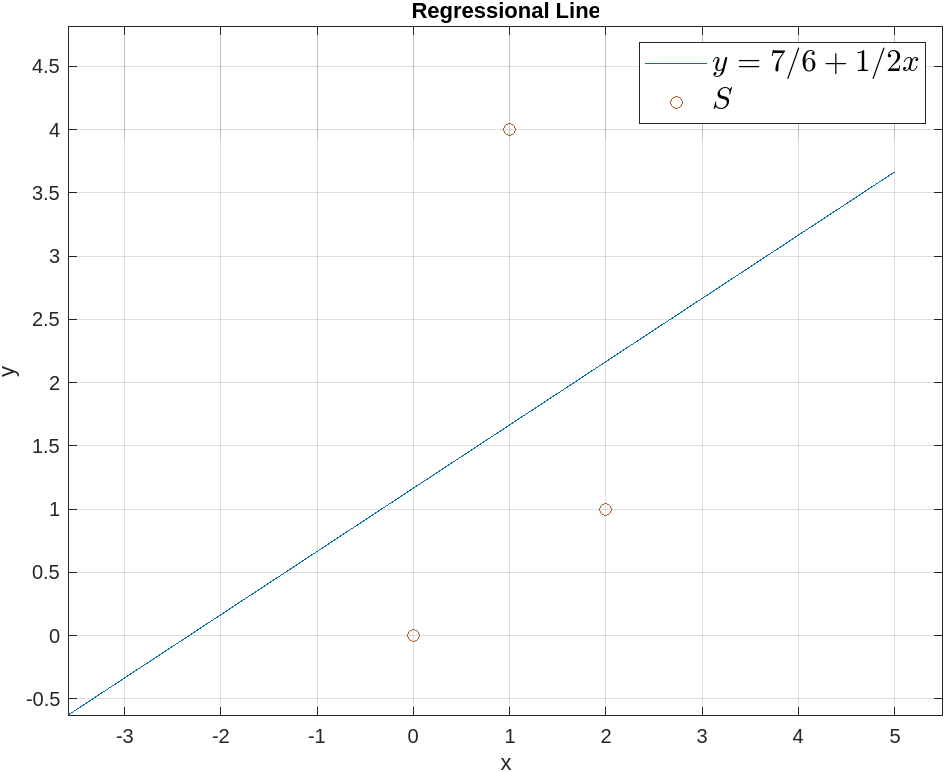
\includegraphics[scale=0.6]{4800A.png}
    \caption{Plot of Regeressional Line $y = \frac{7}{6} + \frac{1}{2}x$}
    \label{fig:my_label}
\end{figure}

\section*{Problem \#5}

Plotting $f(a,b)$ we get,
\begin{figure}[H]
    \centering
    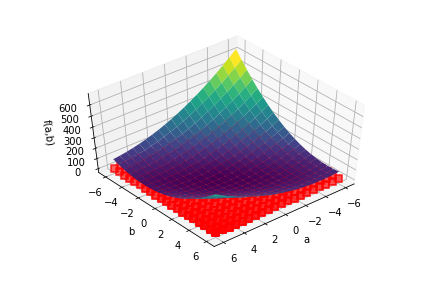
\includegraphics[scale=0.8]{Thatgraph (1).png}
    \caption{Plot of $f(a,b)$}
    \label{fig:my_label}
\end{figure}

Where the plane in red denotes $Z = f\left(\frac{7}{6}, \frac{1}{2}\right)$
\end{document} 